%=============================================================================
% SPATIAL ANALYSIS SECTION
% For inclusion in main NeurIPS 2025 document
%=============================================================================
%
% USAGE: Add %=============================================================================
% SPATIAL ANALYSIS SECTION
% For inclusion in main NeurIPS 2025 document
%=============================================================================
%
% USAGE: Add %=============================================================================
% SPATIAL ANALYSIS SECTION
% For inclusion in main NeurIPS 2025 document
%=============================================================================
%
% USAGE: Add %=============================================================================
% SPATIAL ANALYSIS SECTION
% For inclusion in main NeurIPS 2025 document
%=============================================================================
%
% USAGE: Add \input{spatial_analysis_section} in your Results section
%
% REQUIRED PACKAGES - Add these to your main.tex preamble:
%   \usepackage{siunitx}
%
% REQUIRED FILES:
%   figures/mechanistic_analysis.pdf (or .png)
%
% Note: booktabs, multirow, graphicx are already in your main.tex
%=============================================================================

\subsection{Mechanistic Analysis of Spatial Reasoning}
\label{sec:mechanistic}

Beyond aggregate accuracy metrics, we seek to understand \textit{why} models succeed or fail at spatial reasoning. To this end, we conduct mechanistic analysis on Qwen2.5-VL-7B (8.29B parameters), extracting internal activations and attention patterns to identify neural correlates of correct spatial reasoning.

\paragraph{Method.}

We evaluate Qwen2.5-VL-7B on 50 COCO images, generating \num{3672} spatial queries that span all task types, frame types, and relation axes defined in our benchmark. Table~\ref{tab:qwen_eval} summarizes the results: the model achieves 63.9\% accuracy on egocentric tasks but only 52.8\% on allocentric tasks, confirming an 11.1 percentage point gap that indicates perspective transformation poses substantial difficulty.

\begin{table}[h]
\centering
\small
\caption{Qwen2.5-VL-7B spatial reasoning accuracy on \num{3672} queries across 50 COCO images.}
\label{tab:qwen_eval}
\begin{tabular}{@{}lcc@{}}
\toprule
\textbf{Task Type} & \textbf{Accuracy (\%)} & \textbf{Correct / Total} \\
\midrule
Egocentric  & 63.9 & 1477 / 2312 \\
Allocentric & 52.8 & 718 / 1360 \\
\midrule
\textbf{Overall} & \textbf{59.8} & \textbf{2195 / 3672} \\
\bottomrule
\end{tabular}
\end{table}

To probe the internal mechanisms underlying these accuracy differences, we sample 33 cases---17 correct and 16 incorrect predictions---and extract two complementary signals. First, we compute \textit{activation norms} (L2 norm of hidden states) at each layer, measuring representation strength. Second, we compute the \textit{image attention ratio}, defined as the fraction of attention weights directed to image tokens versus text tokens, quantifying how strongly the model grounds its reasoning in visual content.

\paragraph{Results.}

Figure~\ref{fig:mechanistic} presents our findings across three panels. Panel~(A) shows activation norms across the model's layers, from early vision blocks through the language model. Notably, success and failure cases exhibit nearly identical activation patterns throughout the network, indicating that raw representation magnitude does not differentiate correct from incorrect predictions. This null result is informative: it suggests that failures do not stem from weak or degraded representations, but rather from how those representations are used.

\begin{figure}[t]
\centering
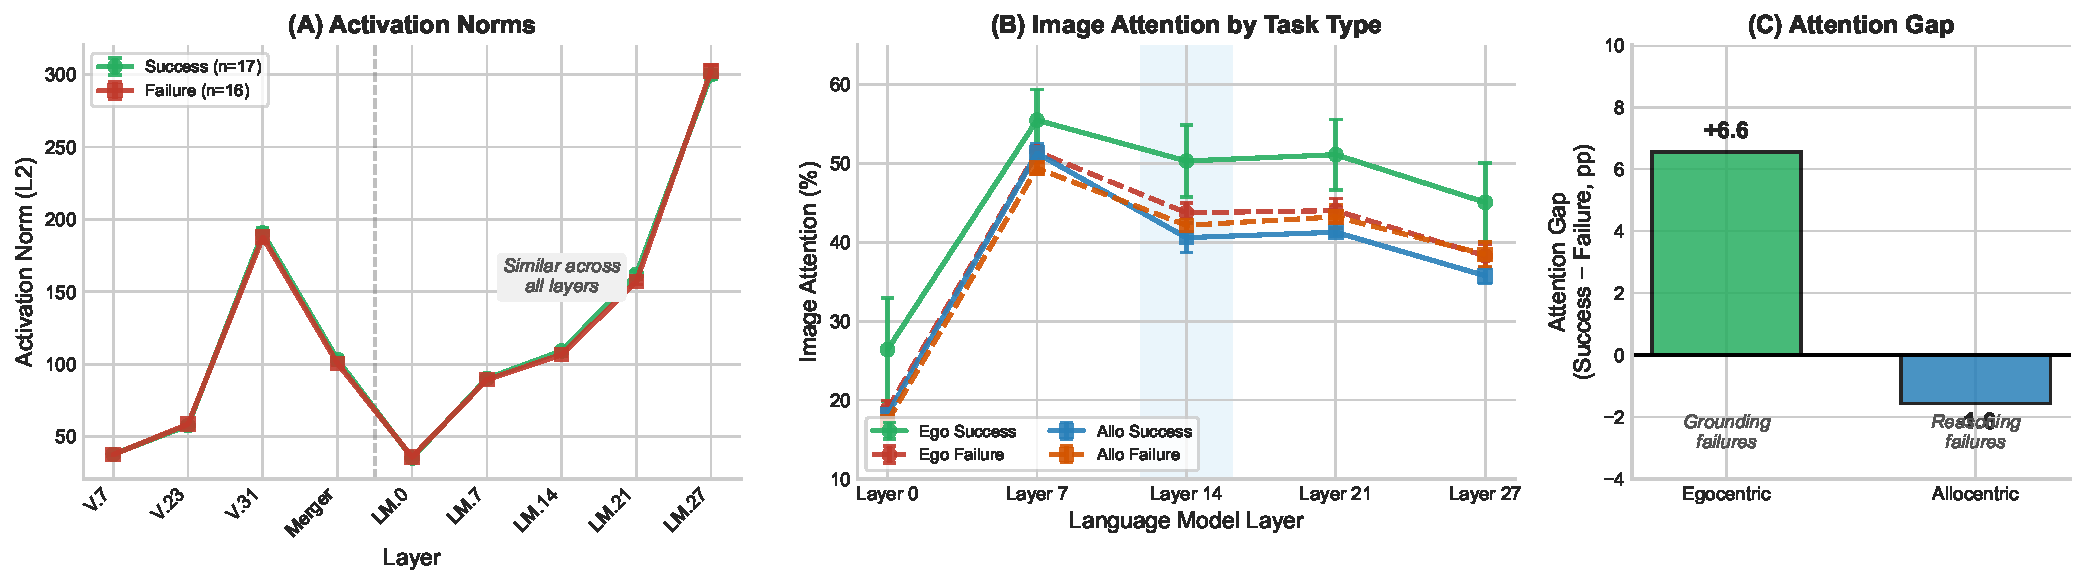
\includegraphics[width=\linewidth]{figures/mechanistic_analysis.pdf}
\caption{\textbf{Mechanistic analysis of spatial reasoning.} (A)~Activation norms show no difference between success and failure cases across all layers, indicating that representation strength alone does not predict correctness. (B)~Image attention ratio reveals task-specific patterns: egocentric success cases (green solid) consistently attend more to image tokens than failures (red dashed), while allocentric cases show no such separation. (C)~At Layer~14, egocentric tasks exhibit a +6.6 percentage point attention advantage for successful predictions (grounding failures), whereas allocentric tasks show --1.6 percentage points (reasoning failures).}
\label{fig:mechanistic}
\end{figure}

The key differentiation emerges in attention patterns, shown in Panel~(B). For egocentric tasks, a clear separation appears: successful predictions (green solid line) consistently maintain higher image attention than failures (red dashed line) across all language model layers, with the gap most pronounced at Layer~14. In contrast, allocentric tasks show no such separation---the success and failure lines interleave throughout the network, with successful predictions sometimes showing \textit{lower} image attention than failures.

Panel~(C) quantifies this divergence at Layer~14. For egocentric tasks, successful predictions exhibit 6.6 percentage points higher image attention than failures (50.3\% vs.\ 43.8\%). This pattern indicates that egocentric failures are fundamentally \textit{grounding failures}---the model does not sufficiently attend to visual content when it answers incorrectly. For allocentric tasks, successful predictions show 1.6 percentage points \textit{lower} attention to image tokens than failures (40.6\% vs.\ 42.2\%). This reversal indicates that allocentric failures are \textit{reasoning failures}: the model attends to the image adequately but cannot correctly perform the perspective transformation required to answer from an object's viewpoint.

\paragraph{Takeaways.}

These findings reveal that spatial reasoning failures arise from fundamentally different mechanisms depending on task type. The similarity in activation norms rules out representation degradation as a failure mode; instead, the divergence appears in how attention is allocated. For egocentric reasoning, success correlates with stronger visual grounding, suggesting that attention-focused training or architectural modifications could yield improvements. For allocentric reasoning, however, the absence of an attention deficit points to a deeper limitation in perspective-taking capabilities, which may require explicit modules or training objectives that teach reference frame transformation.
 in your Results section
%
% REQUIRED PACKAGES - Add these to your main.tex preamble:
%   \usepackage{siunitx}
%
% REQUIRED FILES:
%   figures/mechanistic_analysis.pdf (or .png)
%
% Note: booktabs, multirow, graphicx are already in your main.tex
%=============================================================================

\subsection{Mechanistic Analysis of Spatial Reasoning}
\label{sec:mechanistic}

Beyond aggregate accuracy metrics, we seek to understand \textit{why} models succeed or fail at spatial reasoning. To this end, we conduct mechanistic analysis on Qwen2.5-VL-7B (8.29B parameters), extracting internal activations and attention patterns to identify neural correlates of correct spatial reasoning.

\paragraph{Method.}

We evaluate Qwen2.5-VL-7B on 50 COCO images, generating \num{3672} spatial queries that span all task types, frame types, and relation axes defined in our benchmark. Table~\ref{tab:qwen_eval} summarizes the results: the model achieves 63.9\% accuracy on egocentric tasks but only 52.8\% on allocentric tasks, confirming an 11.1 percentage point gap that indicates perspective transformation poses substantial difficulty.

\begin{table}[h]
\centering
\small
\caption{Qwen2.5-VL-7B spatial reasoning accuracy on \num{3672} queries across 50 COCO images.}
\label{tab:qwen_eval}
\begin{tabular}{@{}lcc@{}}
\toprule
\textbf{Task Type} & \textbf{Accuracy (\%)} & \textbf{Correct / Total} \\
\midrule
Egocentric  & 63.9 & 1477 / 2312 \\
Allocentric & 52.8 & 718 / 1360 \\
\midrule
\textbf{Overall} & \textbf{59.8} & \textbf{2195 / 3672} \\
\bottomrule
\end{tabular}
\end{table}

To probe the internal mechanisms underlying these accuracy differences, we sample 33 cases---17 correct and 16 incorrect predictions---and extract two complementary signals. First, we compute \textit{activation norms} (L2 norm of hidden states) at each layer, measuring representation strength. Second, we compute the \textit{image attention ratio}, defined as the fraction of attention weights directed to image tokens versus text tokens, quantifying how strongly the model grounds its reasoning in visual content.

\paragraph{Results.}

Figure~\ref{fig:mechanistic} presents our findings across three panels. Panel~(A) shows activation norms across the model's layers, from early vision blocks through the language model. Notably, success and failure cases exhibit nearly identical activation patterns throughout the network, indicating that raw representation magnitude does not differentiate correct from incorrect predictions. This null result is informative: it suggests that failures do not stem from weak or degraded representations, but rather from how those representations are used.

\begin{figure}[t]
\centering
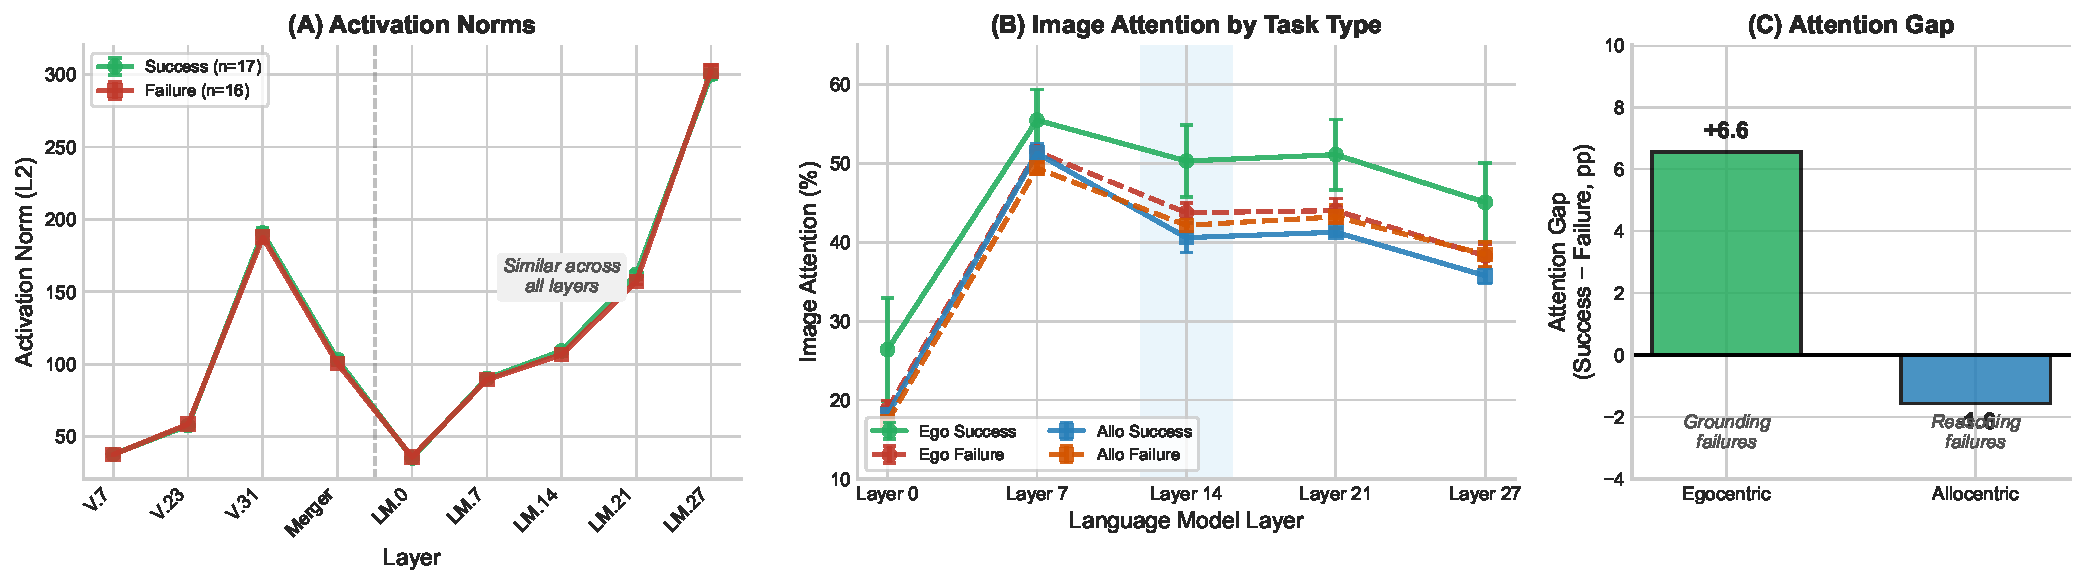
\includegraphics[width=\linewidth]{figures/mechanistic_analysis.pdf}
\caption{\textbf{Mechanistic analysis of spatial reasoning.} (A)~Activation norms show no difference between success and failure cases across all layers, indicating that representation strength alone does not predict correctness. (B)~Image attention ratio reveals task-specific patterns: egocentric success cases (green solid) consistently attend more to image tokens than failures (red dashed), while allocentric cases show no such separation. (C)~At Layer~14, egocentric tasks exhibit a +6.6 percentage point attention advantage for successful predictions (grounding failures), whereas allocentric tasks show --1.6 percentage points (reasoning failures).}
\label{fig:mechanistic}
\end{figure}

The key differentiation emerges in attention patterns, shown in Panel~(B). For egocentric tasks, a clear separation appears: successful predictions (green solid line) consistently maintain higher image attention than failures (red dashed line) across all language model layers, with the gap most pronounced at Layer~14. In contrast, allocentric tasks show no such separation---the success and failure lines interleave throughout the network, with successful predictions sometimes showing \textit{lower} image attention than failures.

Panel~(C) quantifies this divergence at Layer~14. For egocentric tasks, successful predictions exhibit 6.6 percentage points higher image attention than failures (50.3\% vs.\ 43.8\%). This pattern indicates that egocentric failures are fundamentally \textit{grounding failures}---the model does not sufficiently attend to visual content when it answers incorrectly. For allocentric tasks, successful predictions show 1.6 percentage points \textit{lower} attention to image tokens than failures (40.6\% vs.\ 42.2\%). This reversal indicates that allocentric failures are \textit{reasoning failures}: the model attends to the image adequately but cannot correctly perform the perspective transformation required to answer from an object's viewpoint.

\paragraph{Takeaways.}

These findings reveal that spatial reasoning failures arise from fundamentally different mechanisms depending on task type. The similarity in activation norms rules out representation degradation as a failure mode; instead, the divergence appears in how attention is allocated. For egocentric reasoning, success correlates with stronger visual grounding, suggesting that attention-focused training or architectural modifications could yield improvements. For allocentric reasoning, however, the absence of an attention deficit points to a deeper limitation in perspective-taking capabilities, which may require explicit modules or training objectives that teach reference frame transformation.
 in your Results section
%
% REQUIRED PACKAGES - Add these to your main.tex preamble:
%   \usepackage{siunitx}
%
% REQUIRED FILES:
%   figures/mechanistic_analysis.pdf (or .png)
%
% Note: booktabs, multirow, graphicx are already in your main.tex
%=============================================================================

\subsection{Mechanistic Analysis of Spatial Reasoning}
\label{sec:mechanistic}

Beyond aggregate accuracy metrics, we seek to understand \textit{why} models succeed or fail at spatial reasoning. To this end, we conduct mechanistic analysis on Qwen2.5-VL-7B (8.29B parameters), extracting internal activations and attention patterns to identify neural correlates of correct spatial reasoning.

\paragraph{Method.}

We evaluate Qwen2.5-VL-7B on 50 COCO images, generating \num{3672} spatial queries that span all task types, frame types, and relation axes defined in our benchmark. Table~\ref{tab:qwen_eval} summarizes the results: the model achieves 63.9\% accuracy on egocentric tasks but only 52.8\% on allocentric tasks, confirming an 11.1 percentage point gap that indicates perspective transformation poses substantial difficulty.

\begin{table}[h]
\centering
\small
\caption{Qwen2.5-VL-7B spatial reasoning accuracy on \num{3672} queries across 50 COCO images.}
\label{tab:qwen_eval}
\begin{tabular}{@{}lcc@{}}
\toprule
\textbf{Task Type} & \textbf{Accuracy (\%)} & \textbf{Correct / Total} \\
\midrule
Egocentric  & 63.9 & 1477 / 2312 \\
Allocentric & 52.8 & 718 / 1360 \\
\midrule
\textbf{Overall} & \textbf{59.8} & \textbf{2195 / 3672} \\
\bottomrule
\end{tabular}
\end{table}

To probe the internal mechanisms underlying these accuracy differences, we sample 33 cases---17 correct and 16 incorrect predictions---and extract two complementary signals. First, we compute \textit{activation norms} (L2 norm of hidden states) at each layer, measuring representation strength. Second, we compute the \textit{image attention ratio}, defined as the fraction of attention weights directed to image tokens versus text tokens, quantifying how strongly the model grounds its reasoning in visual content.

\paragraph{Results.}

Figure~\ref{fig:mechanistic} presents our findings across three panels. Panel~(A) shows activation norms across the model's layers, from early vision blocks through the language model. Notably, success and failure cases exhibit nearly identical activation patterns throughout the network, indicating that raw representation magnitude does not differentiate correct from incorrect predictions. This null result is informative: it suggests that failures do not stem from weak or degraded representations, but rather from how those representations are used.

\begin{figure}[t]
\centering
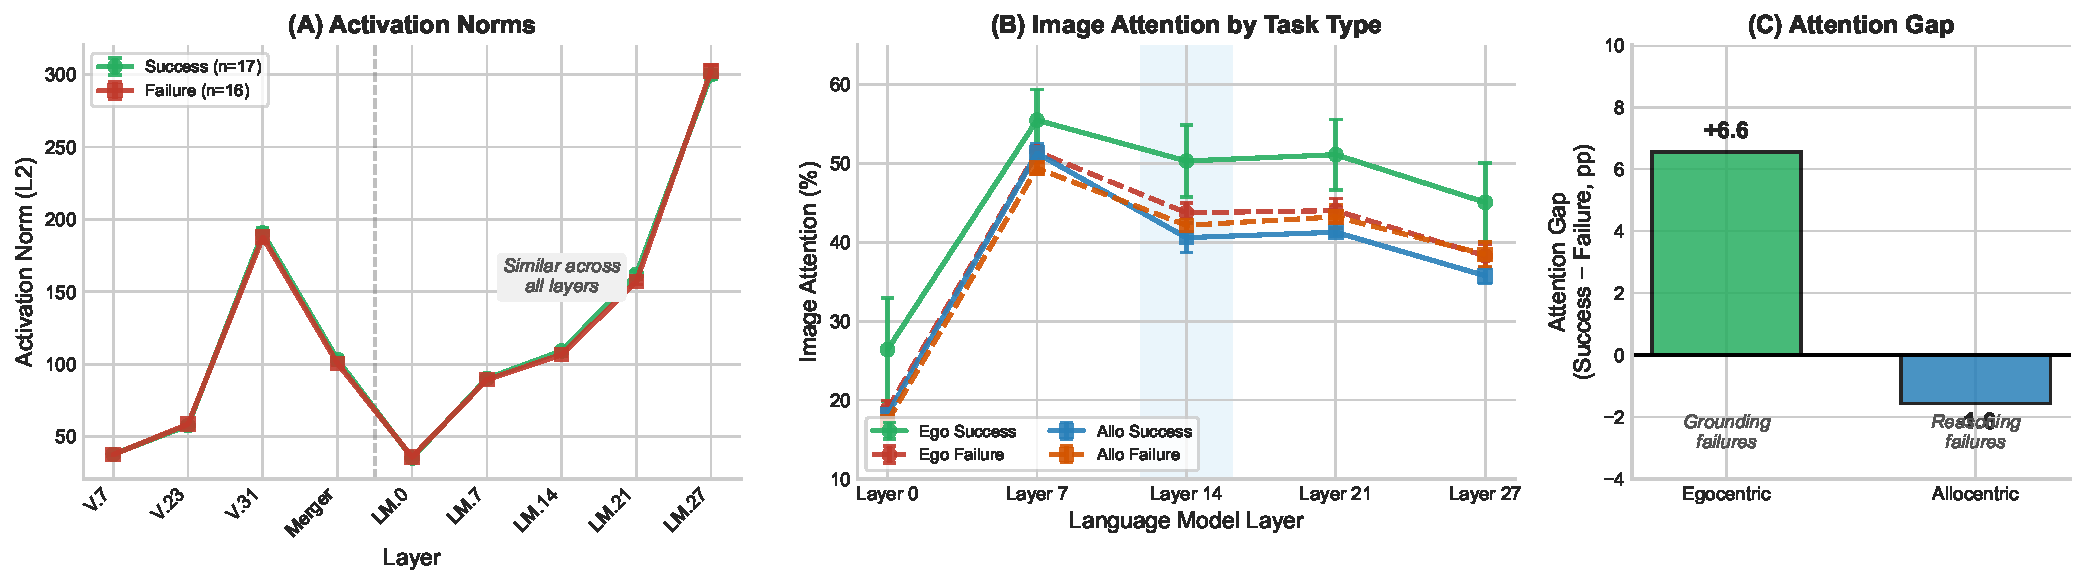
\includegraphics[width=\linewidth]{figures/mechanistic_analysis.pdf}
\caption{\textbf{Mechanistic analysis of spatial reasoning.} (A)~Activation norms show no difference between success and failure cases across all layers, indicating that representation strength alone does not predict correctness. (B)~Image attention ratio reveals task-specific patterns: egocentric success cases (green solid) consistently attend more to image tokens than failures (red dashed), while allocentric cases show no such separation. (C)~At Layer~14, egocentric tasks exhibit a +6.6 percentage point attention advantage for successful predictions (grounding failures), whereas allocentric tasks show --1.6 percentage points (reasoning failures).}
\label{fig:mechanistic}
\end{figure}

The key differentiation emerges in attention patterns, shown in Panel~(B). For egocentric tasks, a clear separation appears: successful predictions (green solid line) consistently maintain higher image attention than failures (red dashed line) across all language model layers, with the gap most pronounced at Layer~14. In contrast, allocentric tasks show no such separation---the success and failure lines interleave throughout the network, with successful predictions sometimes showing \textit{lower} image attention than failures.

Panel~(C) quantifies this divergence at Layer~14. For egocentric tasks, successful predictions exhibit 6.6 percentage points higher image attention than failures (50.3\% vs.\ 43.8\%). This pattern indicates that egocentric failures are fundamentally \textit{grounding failures}---the model does not sufficiently attend to visual content when it answers incorrectly. For allocentric tasks, successful predictions show 1.6 percentage points \textit{lower} attention to image tokens than failures (40.6\% vs.\ 42.2\%). This reversal indicates that allocentric failures are \textit{reasoning failures}: the model attends to the image adequately but cannot correctly perform the perspective transformation required to answer from an object's viewpoint.

\paragraph{Takeaways.}

These findings reveal that spatial reasoning failures arise from fundamentally different mechanisms depending on task type. The similarity in activation norms rules out representation degradation as a failure mode; instead, the divergence appears in how attention is allocated. For egocentric reasoning, success correlates with stronger visual grounding, suggesting that attention-focused training or architectural modifications could yield improvements. For allocentric reasoning, however, the absence of an attention deficit points to a deeper limitation in perspective-taking capabilities, which may require explicit modules or training objectives that teach reference frame transformation.
 in your Results section
%
% REQUIRED PACKAGES - Add these to your main.tex preamble:
%   \usepackage{siunitx}
%
% REQUIRED FILES:
%   figures/mechanistic_analysis.pdf (or .png)
%
% Note: booktabs, multirow, graphicx are already in your main.tex
%=============================================================================

\subsection{Mechanistic Analysis of Spatial Reasoning}
\label{sec:mechanistic}

Beyond aggregate accuracy metrics, we seek to understand \textit{why} models succeed or fail at spatial reasoning. To this end, we conduct mechanistic analysis on Qwen2.5-VL-7B (8.29B parameters), extracting internal activations and attention patterns to identify neural correlates of correct spatial reasoning.

\paragraph{Method.}

We evaluate Qwen2.5-VL-7B on 50 COCO images, generating \num{3672} spatial queries that span all task types, frame types, and relation axes defined in our benchmark. Table~\ref{tab:qwen_eval} summarizes the results: the model achieves 63.9\% accuracy on egocentric tasks but only 52.8\% on allocentric tasks, confirming an 11.1 percentage point gap that indicates perspective transformation poses substantial difficulty.

\begin{table}[h]
\centering
\small
\caption{Qwen2.5-VL-7B spatial reasoning accuracy on \num{3672} queries across 50 COCO images.}
\label{tab:qwen_eval}
\begin{tabular}{@{}lcc@{}}
\toprule
\textbf{Task Type} & \textbf{Accuracy (\%)} & \textbf{Correct / Total} \\
\midrule
Egocentric  & 63.9 & 1477 / 2312 \\
Allocentric & 52.8 & 718 / 1360 \\
\midrule
\textbf{Overall} & \textbf{59.8} & \textbf{2195 / 3672} \\
\bottomrule
\end{tabular}
\end{table}

To probe the internal mechanisms underlying these accuracy differences, we sample 33 cases---17 correct and 16 incorrect predictions---and extract two complementary signals. First, we compute \textit{activation norms} (L2 norm of hidden states) at each layer, measuring representation strength. Second, we compute the \textit{image attention ratio}, defined as the fraction of attention weights directed to image tokens versus text tokens, quantifying how strongly the model grounds its reasoning in visual content.

\paragraph{Results.}

Figure~\ref{fig:mechanistic} presents our findings across three panels. Panel~(A) shows activation norms across the model's layers, from early vision blocks through the language model. Notably, success and failure cases exhibit nearly identical activation patterns throughout the network, indicating that raw representation magnitude does not differentiate correct from incorrect predictions. This null result is informative: it suggests that failures do not stem from weak or degraded representations, but rather from how those representations are used.

\begin{figure}[t]
\centering
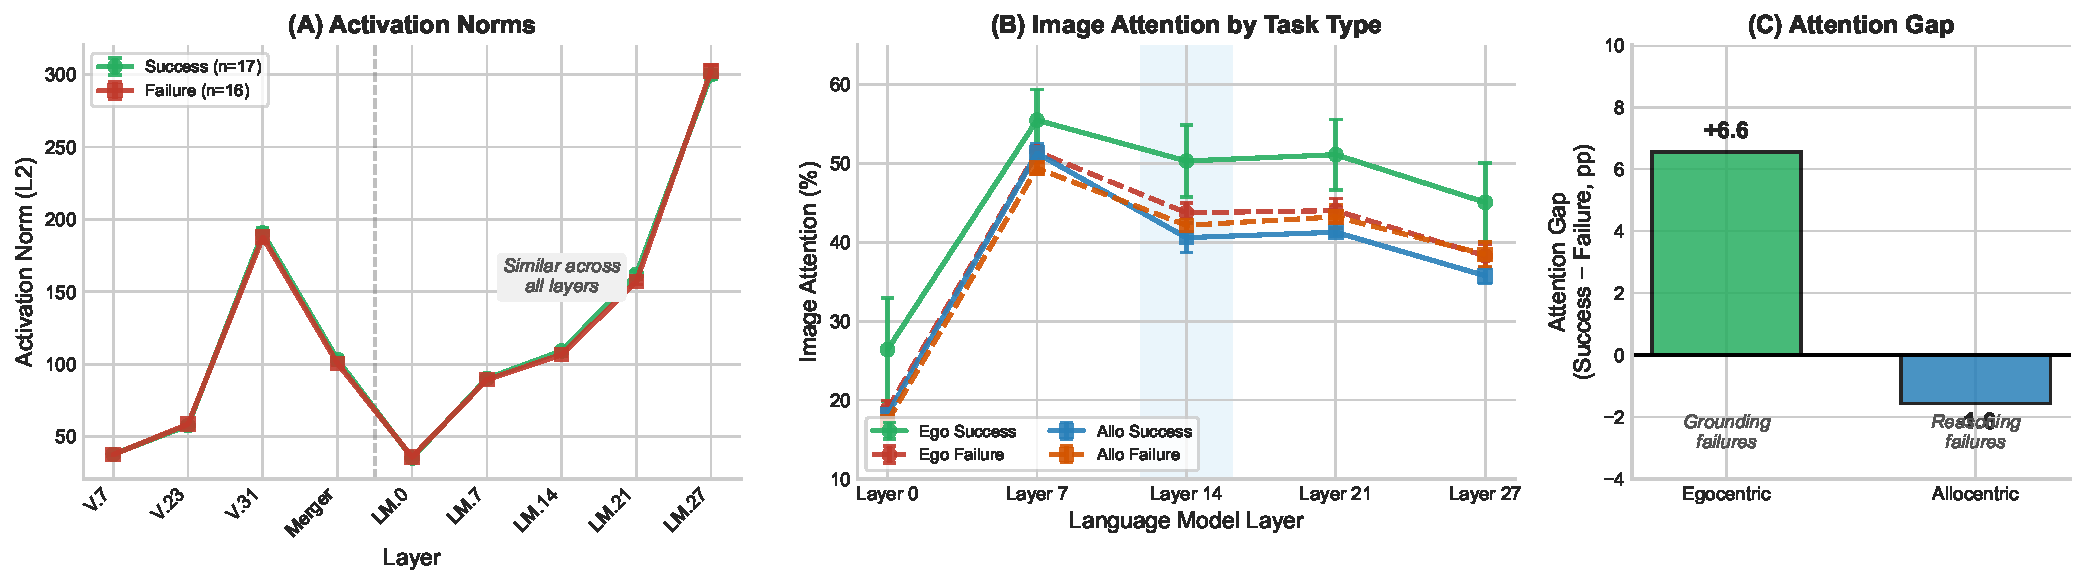
\includegraphics[width=\linewidth]{figures/mechanistic_analysis.pdf}
\caption{\textbf{Mechanistic analysis of spatial reasoning.} (A)~Activation norms show no difference between success and failure cases across all layers, indicating that representation strength alone does not predict correctness. (B)~Image attention ratio reveals task-specific patterns: egocentric success cases (green solid) consistently attend more to image tokens than failures (red dashed), while allocentric cases show no such separation. (C)~At Layer~14, egocentric tasks exhibit a +6.6 percentage point attention advantage for successful predictions (grounding failures), whereas allocentric tasks show --1.6 percentage points (reasoning failures).}
\label{fig:mechanistic}
\end{figure}

The key differentiation emerges in attention patterns, shown in Panel~(B). For egocentric tasks, a clear separation appears: successful predictions (green solid line) consistently maintain higher image attention than failures (red dashed line) across all language model layers, with the gap most pronounced at Layer~14. In contrast, allocentric tasks show no such separation---the success and failure lines interleave throughout the network, with successful predictions sometimes showing \textit{lower} image attention than failures.

Panel~(C) quantifies this divergence at Layer~14. For egocentric tasks, successful predictions exhibit 6.6 percentage points higher image attention than failures (50.3\% vs.\ 43.8\%). This pattern indicates that egocentric failures are fundamentally \textit{grounding failures}---the model does not sufficiently attend to visual content when it answers incorrectly. For allocentric tasks, successful predictions show 1.6 percentage points \textit{lower} attention to image tokens than failures (40.6\% vs.\ 42.2\%). This reversal indicates that allocentric failures are \textit{reasoning failures}: the model attends to the image adequately but cannot correctly perform the perspective transformation required to answer from an object's viewpoint.

\paragraph{Takeaways.}

These findings reveal that spatial reasoning failures arise from fundamentally different mechanisms depending on task type. The similarity in activation norms rules out representation degradation as a failure mode; instead, the divergence appears in how attention is allocated. For egocentric reasoning, success correlates with stronger visual grounding, suggesting that attention-focused training or architectural modifications could yield improvements. For allocentric reasoning, however, the absence of an attention deficit points to a deeper limitation in perspective-taking capabilities, which may require explicit modules or training objectives that teach reference frame transformation.
